The frontend is a software tool designed  to  provide  an  easy way for users to
model complicated  behaviours of photovoltaic modules. The software communicates
with the device via  a  USB  cable at real-time, which means any changes made in
the tool have  an  immediate  effect  on  the  generated  output  voltage of the
hardware device itself.

The frontend was  built  using  the Qt framework\cite{ref:qt}, Qwt\cite{ref:qwt}
for 2D plots and QwtPlot3D\cite{ref:qwtplot3d} for 3D  plots, and was written in
C++.  Qt  was  chosen because it supports all major platforms  and  has  a  very
powerful set of graphical components. Its Graphical User Interface (GUI) can  be
seen  in  figure \ref{fig:frontend:screenshot}. On the left side is  a  list  of
cells and their parameters. Cells  can be removed or added, and their individual
parameters  (open  circuit  voltage,  short  circuit current, dark  voltage  and
irradiation) can be modified -- the  effects  of which are immediate, as already
mentioned. A 2D plot shows what the currently  active  I-V  characteristic curve
looks like, along  with  its  corresponding  power  curve.  A  3D plot shows the
behaviour  of  the  2D power curve in function with irradiation. In the top left
corner  of  the  GUI  the actual measured voltage and current of the  device  is
displayed.

\begin{figure}[th!]
    \centering
    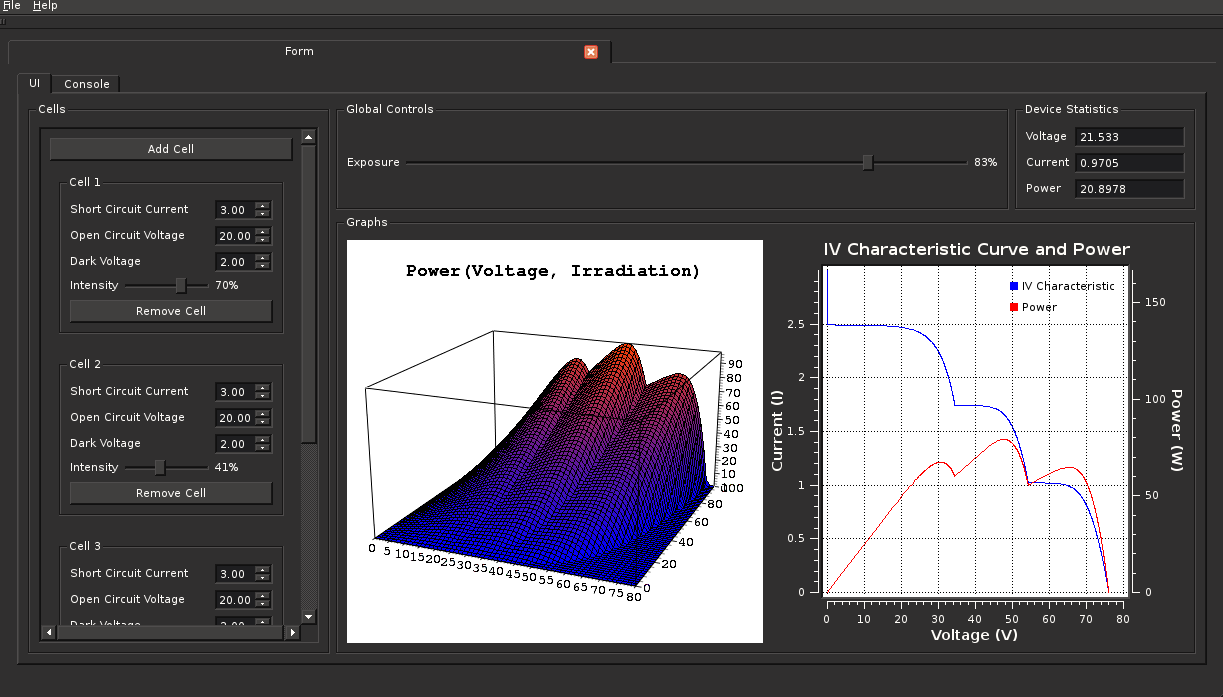
\includegraphics[width=.8\textwidth]{images/frontend/frontend.png}
    \caption{Screen-shot of the frontend's Graphical User Interface (GUI)}
    \label{fig:frontend:screenshot}
\end{figure}

